\documentclass[tikz]{standalone}

\begin{document}
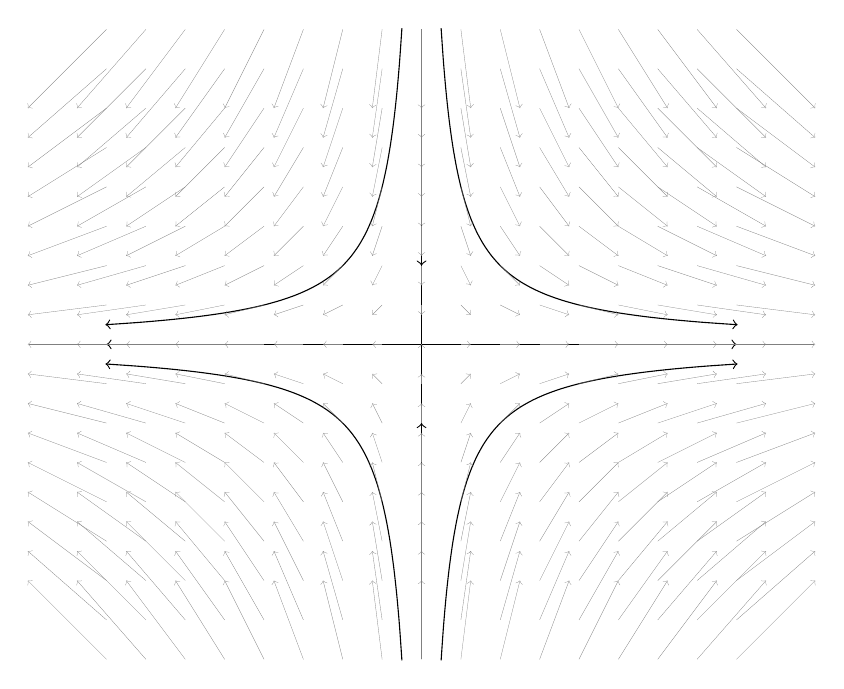
\begin{tikzpicture}
\draw (-4, 0) -- (4, 0);
\draw (0, -4) -- (0, 4);
\draw[->] (0, -4) -- (0, -1);
\draw[->] (0, 4) -- (0, 1);
\draw[->] (1, 0) -- (4, 0);
\draw[->] (-1, 0) -- (-4, 0);

\draw[->, domain=-1.39:1.39, smooth] 
  plot ({exp(\x)}, {exp(-\x)});
\draw[->, domain=-1.39:1.39, smooth] 
  plot ({exp(\x)}, {-exp(-\x)});
\draw[->, domain=-1.39:1.39, smooth] 
  plot ({-exp(\x)}, {-exp(-\x)});
\draw[->, domain=-1.39:1.39, smooth] 
  plot ({-exp(\x)}, {exp(-\x)});

\foreach \x in {-4, -3.5, ..., 4} {
  \foreach \y in {-4, -3.5, ..., 4} {
    \draw[->, ultra thin,
      gray] (\x, \y) -- +(0.25 * \x, -
      0.25 * \y);
  }
}
\end{tikzpicture}
\end{document}
